\documentclass{beamer}
% Required packages
\usepackage{amsmath}
\usepackage{physics}
\usepackage{graphicx}
\usepackage{siunitx}
\usepackage{xcolor}
\usepackage{textcomp} % For quotes
\usepackage{csquotes}

% Define custom colors for DS9 theme
\definecolor{ds9blue}{RGB}{25,25,112}
\definecolor{ds9gold}{RGB}{218,165,32}
\definecolor{ds9grey}{RGB}{105,105,105}
\definecolor{ds9red}{RGB}{178,34,34}
% Set up the Madrid theme with custom colors
\usetheme{Madrid}
\usecolortheme{whale}
\setbeamercolor{palette primary}{bg=ds9blue,fg=white}
\setbeamercolor{palette secondary}{bg=ds9grey,fg=white}
\setbeamercolor{palette tertiary}{bg=ds9gold,fg=black}
\setbeamercolor{palette quaternary}{bg=ds9red,fg=white}
\setbeamercolor{structure}{fg=ds9blue}
\setbeamercolor{title}{fg=ds9gold}
\setbeamercolor{subtitle}{fg=ds9gold}
\setbeamercolor{frametitle}{bg=ds9blue,fg=white}
\setbeamercolor{block title}{bg=ds9blue,fg=white}
\setbeamercolor{block body}{bg=ds9grey!20,fg=black}

% Title page configuration
\title[Critical AI Literacy]{AI Literacy}
\subtitle{Addressing LLM Misuse in Educational Settings}
\author[Mr. Gullo]{Mr. Gullo}
\date[April 2025]{April, 2025} % Updated Date

\begin{document}

% Title frame
\begin{frame}
\titlepage
\end{frame}

\begin{frame}{AI Confidence vs Accuracy: XKCD's Take}
  \begin{columns}
    \begin{column}{0.48\textwidth}
     \begin{figure}
        \centering
        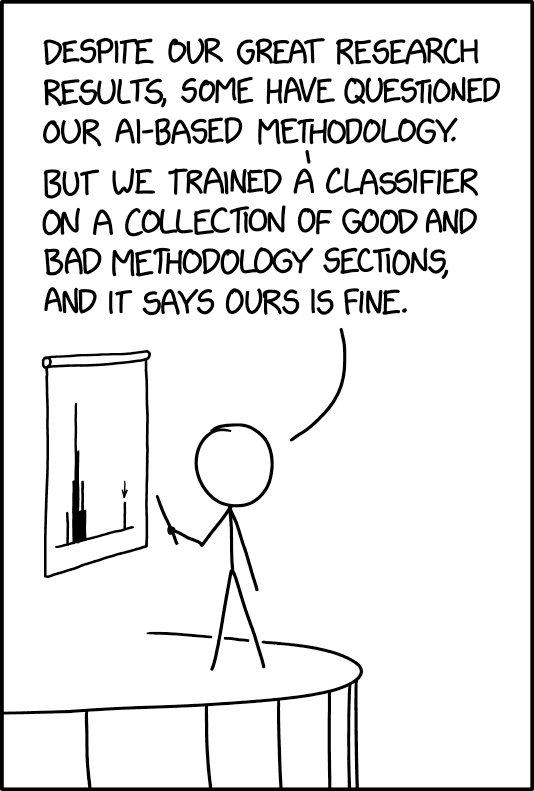
\includegraphics[width=0.6\linewidth]{../src/cs12/images/cs12-ai-methodology.png}
     \caption*{XKCD \#2451: AI Methodology}
      \end{figure}
    \end{column}
    \begin{column}{0.48\textwidth}
      \begin{figure}
          \centering
          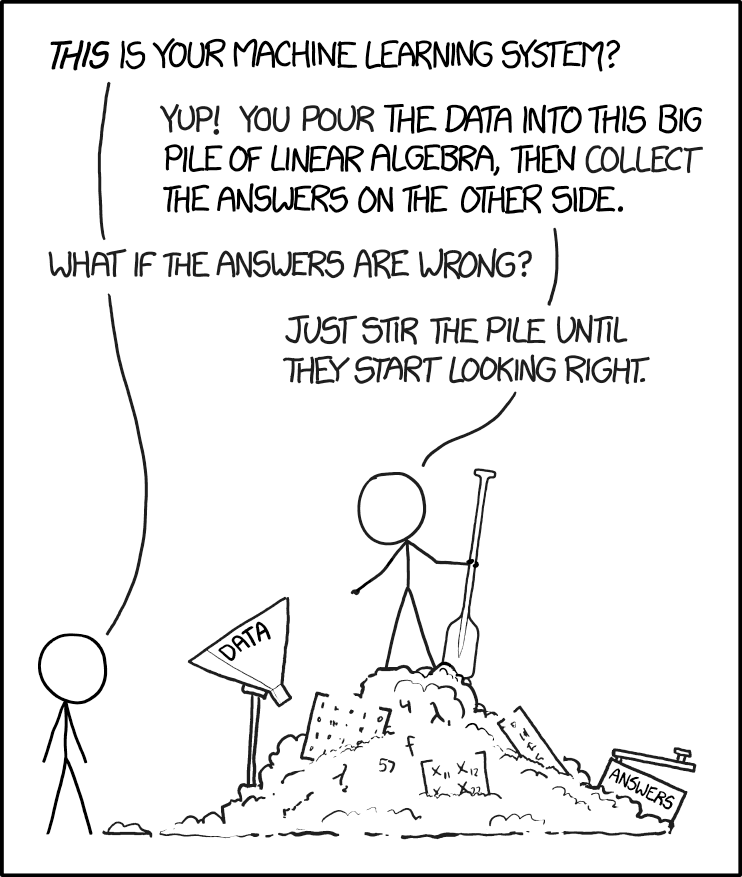
\includegraphics[width=0.8\linewidth]{../src/cs12/images/cs12-ai-machine_learning.png}
                 \caption*{XKCD \#1838: Machine Learning}
      \end{figure}

    \end{column}
  \end{columns}
  \vspace{0.5cm}
  {\tiny Images from xkcd.com by Randall Munroe, used under CC BY-NC license}
\end{frame}

% Learning objectives frame
\begin{frame}{Learning Objectives}
\begin{block}{By the end of this presentation, you will be able to:}
\begin{itemize}
  \item Define LLM hallucinations and explain why they occur
  \item Identify at least three strategies to critically evaluate AI-generated content
  \item Apply principles of effective prompting to improve LLM response quality
  \item Articulate ethical considerations and potential misuse scenarios for academic use of AI tools (based on student data)
\end{itemize}
\end{block}
\end{frame}

% Section frame - Understanding LLM Hallucinations
\section{Understanding LLM Hallucinations}

\begin{frame}{What Are LLM Hallucinations?}
\begin{block}{Definition}
Instances where AI generates content that is:
\begin{itemize}
  \item Factually incorrect | Nonsensical
  \item Disconnected from the input prompt
  \item Yet presented with high confidence
\end{itemize}
\end{block}

\alert{} % Keeps space consistent, maybe remove if not needed
\begin{figure}
    \centering
    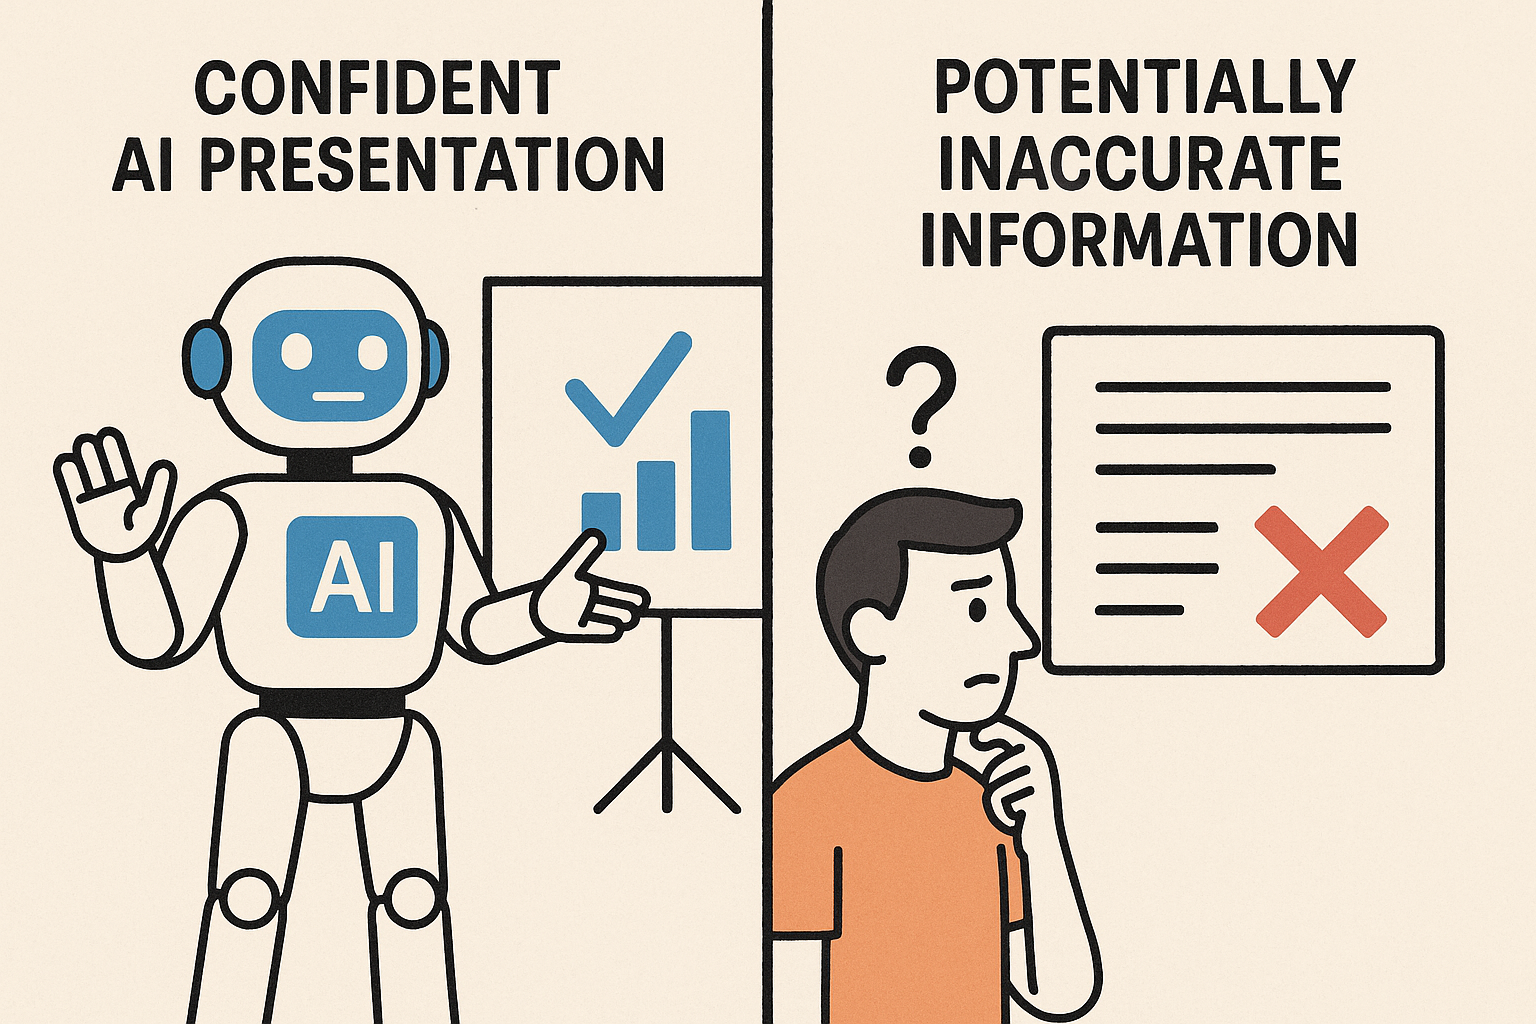
\includegraphics[width=0.5\linewidth]{../src/cs12/images/cs12-ai-hallucination_example.png}
\end{figure}
\end{frame}

% MODIFIED Frame 5: Condensed Version
\begin{frame}{Why Do LLMs Hallucinate?}
\begin{columns}
\column{0.5\textwidth}
\begin{block}{Training Data Issues}
\begin{itemize}
\item Learns from vast, unverified internet text
\item Can reflect biases or be outdated
\end{itemize}
\end{block}
\pause 
\begin{block}{Model Design}
\begin{itemize}
\item Predicts plausible text, not facts
\item Lacks true understanding or reasoning
\end{itemize}
\end{block}
\column{0.5\textwidth}
\pause 
\begin{block}{Prompting Problems}
\begin{itemize}
\item Vague prompts invite fabrication
\item Complex prompts can confuse the AI
\end{itemize}
\end{block}
\pause 
\begin{alertblock}{Key Insight}
LLMs are sophisticated word predictors, not truth tellers!
\end{alertblock}
\end{columns}
\end{frame}

% Section frame - Student Interaction Patterns
\section{Student Interaction Patterns}

% MODIFIED Frame 6: Replaced list with quote
\begin{frame}{How Students Use LLMs: A Key Pattern}

\begin{block}{Dominance of Direct Interaction (Anthropic Report)}
\blockquote{Nearly half (~47\%) of student-AI conversations were Direct—that is, seeking answers or content with minimal engagement.}
\end{block}

% Optional: Keep the graph if space allows and it complements the point.
 \begin{figure}
 \centering
 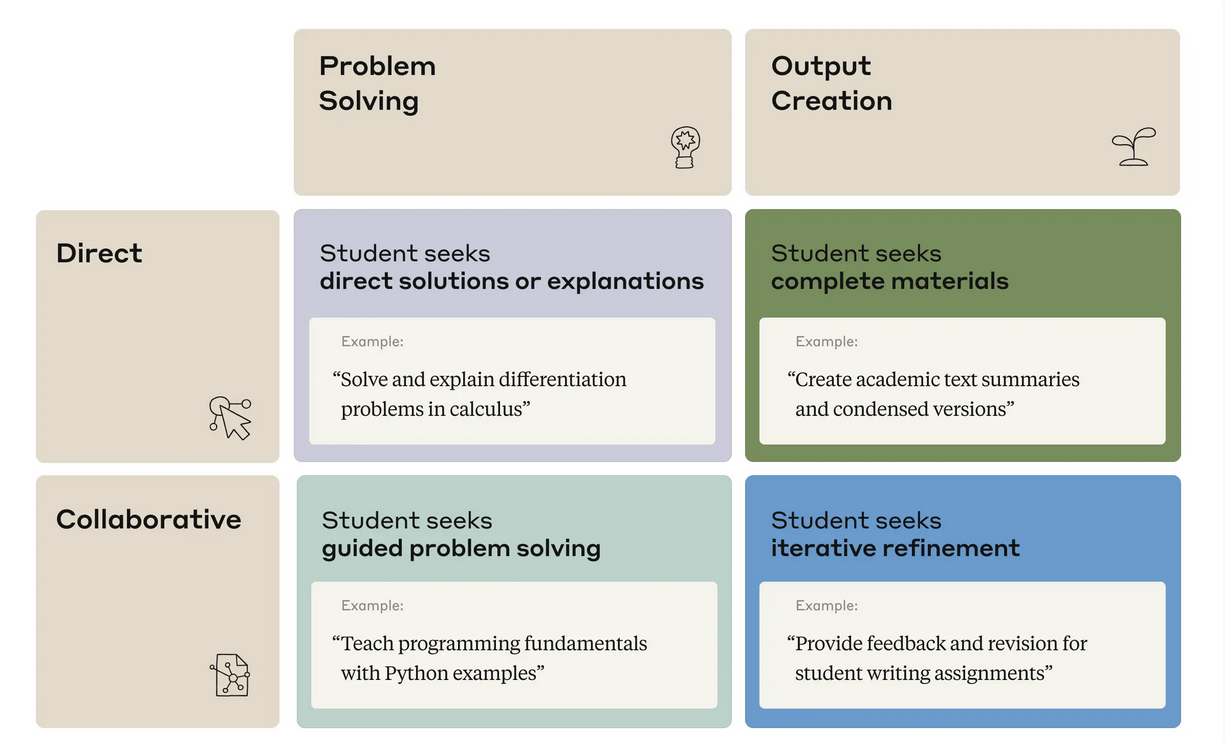
\includegraphics[width=8cm]{../src/cs12/images/cs12-llm-student_interaction_styles.png} %Adjust width as needed
% \caption*{Interaction Styles Distribution}
\end{figure}

\end{frame}

% Frame 7: Discipline-Specific Usage (Kept original, potentially add caption later)
\begin{frame}{Discipline-Specific Usage Patterns}
\begin{block}{Disproportionate Usage by Field}
\begin{itemize}
  \item Computer Science: 36.8\% of conversations (vs. 5.4\% of degrees)
  \item Natural Sciences/Mathematics: 15.2\% (vs. 9.2\%)
  \item Business: 8.9\% (vs. 18.6\%)
  \item Humanities: 6.4\% (vs. 12.5\%)
\end{itemize}
\end{block}
\begin{figure}
    \centering
    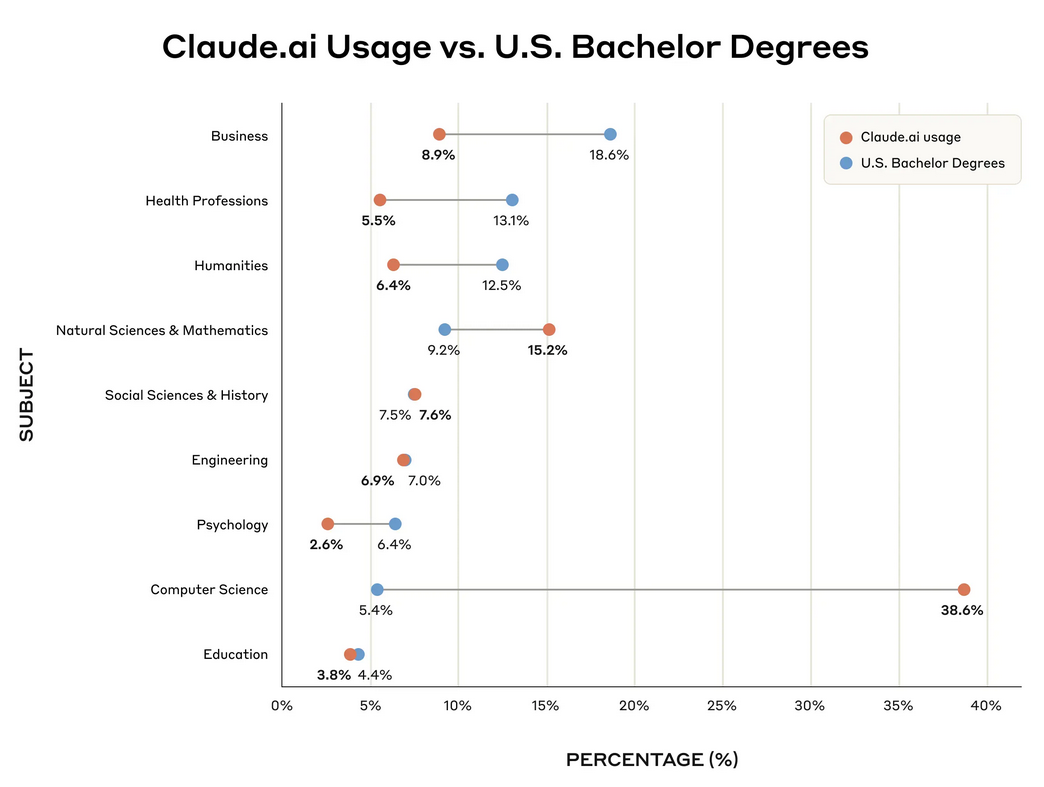
\includegraphics[width=0.5\linewidth]{../src/cs12/images/cs12-llm-discipline_usage.png}
\end{figure}
\end{frame}

% MODIFIED Frame 8: Added quote about offloading tasks
\begin{frame}{Cognitive Functions: Outsourcing Thinking?}

% Text Block First
\begin{block}{Focus on Higher-Order Tasks (Anthropic)}
\begin{itemize}
    \item Creating (39.8\%) \& Analyzing (30.2\%)
\end{itemize}
\end{block}

% Figure Below, potentially wider
\begin{figure}
    \centering
    % Adjust width as desired, e.g., 70% of the total text width
    % % % 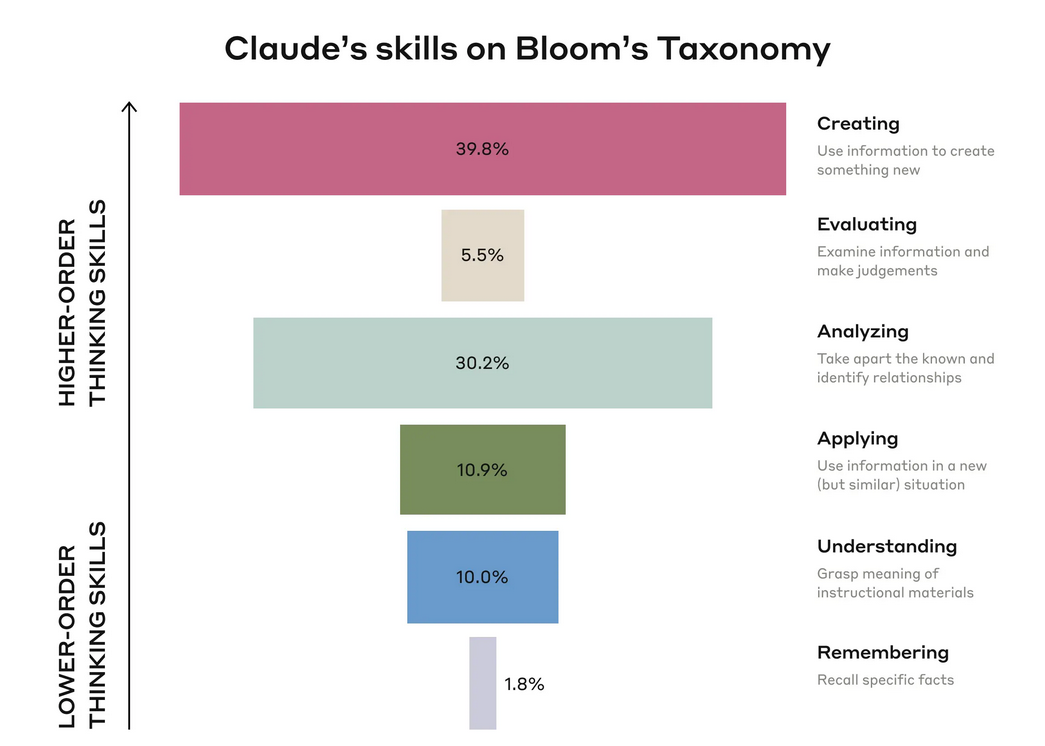
\includegraphics[width=0.6\textwidth]{../images/cs12-llm-blooms_taxonomy.png}
    % Optional: Add caption if desired
    % \caption{Bloom's Taxonomy Levels}
\end{figure}

\end{frame}

% NEW Frame: The Crutch Concern
\begin{frame}{The Concern: AI as a Cognitive Crutch}
\begin{alertblock}{A Core Worry (Anthropic Report)}
\blockquote{...it does point to the potential concerns of students outsourcing cognitive abilities to AI. There are legitimate worries that AI systems may provide a crutch for students, stifling the development of foundational skills needed to support higher-order thinking.}
\end{alertblock}
\end{frame}

% NEW Frame: Specific Misuse Examples
\begin{frame}{Concerning Examples of Misuse (Anthropic Report)}
The study identified direct conversations involving potential academic dishonesty:

\begin{block}{Observed Misuse Cases}
\begin{itemize}
\item \textit{"Provide answers to machine learning multiple-choice questions"}
\item \textit{"Provide direct answers to English language test questions"}
\item \textit{"Rewrite marketing and business texts to avoid plagiarism detection"}
\end{itemize}
\end{block}
\vspace{0.5cm}
\footnotesize{Source: Anthropic Education Report: How University Students Use Claude}
\end{frame}

% Section frame - Learning Implications
\section{Implications for Learning}

% MODIFIED Frame 9: Simplified and integrated quotes
\begin{frame}{Implications for Learning \& Integrity}
\begin{block}{Hindrance to Skill Development}
Over-reliance risks bypassing essential practice in:
\begin{itemize}
    \item Critical thinking \& Information literacy
    \item Foundational knowledge building
\end{itemize}
\blockquote{Concerns exist that AI may provide a crutch... stifling the development of foundational skills.}
\end{block}
\pause  % Optional pause
\begin{block}{Academic Integrity Challenges}
\begin{itemize}
    \item Blurring lines between aid and cheating
    \item Need for clear policies and expectations
\end{itemize}
\blockquote{Even Collaborative conversations... like 'solve probability and statistics homework problems with explanations,'... still offloads significant thinking to the AI.}
\end{block}
\footnotesize{\textit{Quotes adapted/drawn from Anthropic Education Report}}
\end{frame}

% Section frame - Critical Evaluation
\section{Critical Evaluation Strategies}

% MODIFIED Frame 10: Condensed Version
\begin{frame}{Critical Evaluation Strategies}
\begin{columns}
\column{0.5\textwidth}
\begin{block}{Verify Externally}
\begin{itemize}
\item Cross-reference with reliable sources (books, journals)
\item Check AI's cited sources (often fake)
\end{itemize}
\end{block}
\pause 
\begin{block}{Check Internally}
\begin{itemize}
\item Does it answer the prompt logically?
\item Any self-contradictions?
\end{itemize}
\end{block}
\column{0.5\textwidth}
\pause 
\begin{block}{Use Your Judgment}
\begin{itemize}
\item Does it align with your knowledge?
\item "Gut check": Does it seem plausible?
\end{itemize}
\end{block}
\pause 
\begin{block}{Look for Bias}
\begin{itemize}
\item Stereotypes? Generalizations?
\item Lack of diverse views? Loaded words?
\end{itemize}
\end{block}
\end{columns}
\end{frame}

% Section frame - Effective Prompting
\section{Effective Prompting Techniques}

% MODIFIED Frame 11: Condensed Version
\begin{frame}{Principles of Effective Prompting}
\begin{block}{Be Clear and Specific}
Avoid vague requests. State precisely what you need. \\
\textit{Ex: Instead of "Info on climate change," ask "Explain impacts of climate change on Arctic sea ice in the last 50 years, citing findings."}
\end{block}
\pause 
\begin{block}{Provide Context}
Tell the AI the background, your role, and any constraints. \\
\textit{Ex: "I'm a student writing a paper for Bio 101..."}
\end{block}
\pause 
\begin{block}{Define the Output}
Specify desired format, length, tone, or audience. \\
\textit{Ex: "Summarize in 3 bullets" or "Explain for high schoolers."}
\end{block}
\end{frame}

% MODIFIED Frame 12: Condensed Version
\begin{frame}{Advanced Prompting Techniques}
\begin{columns}
\column{0.5\textwidth}
\begin{block}{Few-Shot Prompting}
Provide examples of the desired input/output.
\end{block}
\pause 
\begin{block}{Role Assignment}
Tell the AI to act as an expert, tutor, reviewer, etc.
\end{block}
\column{0.5\textwidth}
\pause 
\begin{block}{Content Grounding}
Instruct AI to base answers *only* on provided text.
\end{block}
\pause 
\begin{block}{Prompt Chaining}
Break complex tasks into smaller, sequential steps.
\end{block}
\end{columns}
\vspace{0.5cm}

\textit{These techniques help guide the AI for better, more focused results.}
\end{frame}

% Examples - I do, We do, You do
\section{Examples}

\begin{frame}{Example 1: Evaluating an LLM Response (Part 1)}

\begin{block}{LLM Generated Statement}
"The Heisenberg Uncertainty Principle states that the more precisely the position of a particle is determined, the less precisely its momentum can be measured. This was experimentally proven in 1927 by Werner Heisenberg using electron diffraction patterns, showing it's impossible to simultaneously know both values with perfect accuracy."
\end{block}

\pause  % Reveal the next block on click

\begin{block}{Claims to Evaluate}
Let's examine the key assertions made:
\begin{enumerate}
  \item The core definition provided?
  \item The claim of experimental proof by Heisenberg in 1927?
  \item The specific method cited (electron diffraction)?
\end{enumerate}
\end{block}

\end{frame}

\begin{frame}{Example 1: Evaluating the Claims (Part 2)}

\begin{itemize}
    \item<1-> \textbf{Claim 1: Definition?} \\
        \textit{Result:} \textbf{Accurate}. The description of the position-momentum trade-off is correct.
    \pause  % Reveal next item on click

    \item<2-> \textbf{Claim 2: Experimental Proof 1927?} \\
        \textit{Result:} \textbf{Error}. Heisenberg derived the principle \emph{theoretically} in 1927. It wasn't based directly on a specific experiment he performed that year.
    \pause  % Reveal next item on click

    \item<3-> \textbf{Claim 3: Method (Electron Diffraction)?} \\
        \textit{Result:} \textbf{Error}. Electron diffraction experiments (like Davisson-Germer, 1927) demonstrated the \emph{wave nature} of electrons, a related but distinct concept. The LLM conflates these.
    \pause  % Reveal final block on click
\end{itemize}

\begin{alertblock}<4->{Conclusion}
The LLM mixed an accurate definition with confident but incorrect historical and experimental details. Verification of specifics is essential.
\end{alertblock}

\end{frame}

% Frame 15: Example 2 (Kept Original)
\begin{frame}{Example 2: "We Do" - Improving a Prompt}
\begin{columns}
\column{0.5\textwidth}
\begin{block}{Original Prompt}
"Tell me about quantum entanglement."
\end{block}
\pause 
\begin{alertblock}{Problems with the Prompt}
\begin{itemize}
  \item Too vague and broad
  \item No context or background
  \item No specified audience/level
  \item No format or structure
\end{itemize}
\end{alertblock}
\pause 
\column{0.5\textwidth}
\begin{block}{Improved Prompt}
"Explain quantum entanglement at a first-year undergraduate physics level. Include:
\begin{itemize}
  \item A clear definition with the key mathematical relationship
  \item One real-world experimental example
  \item Its significance for quantum computing
\end{itemize}
Use simple analogies where appropriate and keep the explanation under 300 words."
\end{block}
\end{columns}
\end{frame}

% Frame 16: Example 3 (Kept Original)
\begin{frame}{Example 3: "You Do" - Creating an AI Policy}
\begin{block}{Scenario}
You are designing a policy for AI use in a physics lab report assignment where students:
\begin{itemize}
  \item Collect experimental data on pendulum motion
  \item Calculate period, uncertainty, and gravitational acceleration
  \item Analyze results and sources of error
  \item Draw conclusions about the accuracy of their measurements
\end{itemize}
\end{block}

\begin{block}{Your Task}
Develop a clear AI policy for this assignment:
\begin{itemize}
  \item Which parts should be
  \textcolor{red}{RED} (AI prohibited)?
  \item Which parts could be
  \textcolor{orange}{ORANGE} (AI permitted with constraints)?
  \item Which parts might be
  \textcolor{green}{GREEN} (AI encouraged)?
  \item What specific disclosure requirements would you include?
\end{itemize}
\end{block}

\begin{alertblock}{Justify your choices based on learning objectives}
What skills do you want students to develop through this assignment?
\end{alertblock}
\end{frame}

% Summary slide
\section{Summary}

% Frame 17: Summary (Kept Original, potentially refine based on new focus)
\begin{frame}{Key Takeaways}
\begin{block}{Critical AI Literacy Framework}
\begin{itemize}
  \item \textbf{Understand} LLM limitations, why hallucinations occur, and potential for misuse
  \item \textbf{Evaluate} AI content critically using multiple verification strategies
  \item \textbf{Prompt} effectively to improve output quality and relevance
  \item \textbf{Apply} clear policies for ethical AI integration, considering learning goals
  \item \textbf{Recognize} the risks of outsourcing critical thinking and skill development
\end{itemize}
\end{block}

\begin{alertblock}{Remember}
LLMs are tools to augment human thinking, not replace it. The ultimate responsibility for the accuracy, integrity, and quality of any work rests with you, not the AI.
\end{alertblock}
\end{frame}

% Frame 18: Questions (Kept Original)
\begin{frame}
\centering
\Huge{Questions?}
\end{frame}

% Frame 19: References (Kept Original)
\begin{frame}{References}
\begin{block}{Key sources}
\begin{itemize}
  \item \href{https://www.anthropic.com/news/anthropic-education-report-how-university-students-use-claude}{Anthropic Education Report: How University Students Use Claude}
  \item \href{https://labelyourdata.com/articles/llm-fine-tuning/llm-hallucination}{LLM Hallucination: Understanding AI Text Errors}
  \item \href{https://www.codecademy.com/article/ai-prompting-best-practices}{AI Prompting Best Practices}
  \item \href{https://libguides.library.arizona.edu/ai-literacy-instructors/verify-facts}{Fact-checking is always needed - AI Literacy in the Age of ChatGPT}
\end{itemize}
\end{block}
\end{frame}

\end{document}